\documentclass[12pt,a4paper]{article}
\usepackage{geometry}
\geometry{margin=1in}
\usepackage{graphicx}
\usepackage{setspace}
\usepackage{titling}
\usepackage{titlesec}
\usepackage{tabularx}
\usepackage{booktabs}
\usepackage{enumitem}
\usepackage{microtype}
\usepackage{newtxtext,newtxmath}
\usepackage[hidelinks]{hyperref}

\titlespacing{\section}{0pt}{0.5em}{0.2em}
\setlength{\parskip}{0.2em}
\setlength{\parindent}{0pt}
\pagenumbering{gobble}

\begin{document}

% --------- COVER PAGE ----------
\begin{titlepage}
    \begin{center}
        \vspace*{0.4cm}
        \includegraphics[width=0.19\textwidth]{Logo_of_Premier_University_(PU).png}\\[0.8cm]
        
        {\fontsize{28}{34}\selectfont \textbf{Premier University}}\\[0.15cm]
        {\fontsize{17}{21}\selectfont Chattogram}\\[0.6cm]

        {\Large \textit{Project Proposal}}\\[0.2cm]

        {\fontsize{18}{24}\selectfont \textbf{Design and Simulation of an IPv6 Smart City IoT Network}}\\[0.08cm]
        {\fontsize{13}{16}\selectfont \textbf{with Quality of Service and Resilient Routing}}\\[0.7cm]

        {\large \textbf{Submitted by}}\\[0.08cm]
\rule{0.21\textwidth}{0.7pt}\\[0.12cm]

\renewcommand{\arraystretch}{1.2}
\begin{tabular}{p{6.5cm} l}
    \textbf{Name} & \textbf{ID} \\
    MD Nishadul Islam Chy Shezan & 0222220005101014 \\
    MD Sakib & 0222220005101019 \\
    Rimjhim Dey & 0222220005101039 \\
\end{tabular}\\[0.6cm]

\begin{center}
    \textbf{Section:} A \\[0.1cm]
    \textbf{Batch:} 42 \\[0.1cm]
    \textbf{Session:} Spring 2025
\end{center}

        {\large \textbf{Submitted to}}\\[0.08cm]
        \rule{0.17\textwidth}{0.7pt}\\[0.11cm]
        {\textbf{Dr. Shahid Md. Asif Iqbal}}\\
        \textit{Professor}\\
        Department of Computer Science and Engineering\\
        \textbf{\textit{Associate Dean}}\\
        Faculty of Engineering\\[0.35cm]

        \vfill
        {\normalsize August 2025}
    \end{center}
\end{titlepage}

% --------- CONTENTS PAGE ----------
\newpage
\begin{center}
    {\Huge \textbf{Contents}}
\end{center}
\vspace{1.5em}

\tableofcontents
\newpage

\pagenumbering{arabic}

% --------- MAIN CONTENT ----------

\section*{Introduction}
\phantomsection
\addcontentsline{toc}{section}{Introduction}
Modern cities deploy a wide range of interconnected sensors to gather valuable data about traffic, air quality, waste management, and infrastructure usage. However, most existing municipal networks still depend heavily on IPv4, which faces serious address limitations and lacks native support for large-scale IoT deployments. This project aims to design a smart city network in Cisco Packet Tracer using IPv6 for virtually unlimited addressing and Quality of Service (QoS) for prioritizing critical emergency traffic.

The proposed network will illustrate how these technologies can improve the reliability, scalability, and responsiveness of city-wide sensor systems, especially under failure scenarios. Current IPv4 constraints—such as address exhaustion requiring complex NAT configurations and limited IoT integration—will be overcome by our hierarchical IPv6 architecture.

\section*{Objectives}
\phantomsection
\addcontentsline{toc}{section}{Objectives}
\begin{enumerate}[label=2.\arabic*, nosep]
    \item Design a scalable smart city network in Cisco Packet Tracer with access, distribution, and core layers
    \item Implement IPv6 across all segments to remove address exhaustion issues
    \item Configure Quality of Service to guarantee priority for emergency traffic
    \item Separate IoT, public Wi-Fi, and administrative devices using VLANs and ACLs
    \item Create automated email alerts through SMTP for critical network events
\end{enumerate}

\section*{Scope}
\phantomsection
\addcontentsline{toc}{section}{Scope}
This project focuses on the design, simulation, and testing of a smart city IoT network prototype in Cisco Packet Tracer. It covers:
\begin{itemize}[nosep]
    \item A robust three-tier network architecture with structured IPv6 addressing
    \item Security enforcement through VLAN segmentation and ACL policies
    \item Deployment of basic network services (SMTP, HTTP) to support system monitoring
    \item Simulation of multiple IoT devices, including traffic sensors, air quality monitors, and smart waste bins
    \item Failover validation and QoS performance testing for critical traffic
\end{itemize}

Physical installation details, advanced encryption frameworks, large-scale application development, and deep real-time analytics platforms are excluded to keep the scope focused on essential networking concepts.

\section*{Tools and Technologies}
\phantomsection
\addcontentsline{toc}{section}{Tools and Technologies}
\textbf{Primary Platform:} Cisco Packet Tracer 8.2.x with IoT device templates and simulation features

\textbf{Networking Protocols:}
\begin{itemize}[nosep]
    \item IPv6 (RFC 8200) for addressing
    \item IEEE 802.1Q for VLAN trunking
\end{itemize}

\textbf{Services:} SMTP, HTTP

\textbf{Security:} Extended ACLs, VLAN segmentation, port security for device control

\newpage
\section*{Key Features}
\phantomsection
\addcontentsline{toc}{section}{Key Features}
\begin{enumerate}[label=5.\arabic*, nosep]
    \item \textbf{IPv6 Implementation:} Fully native IPv6 addressing with /48 for sites and /64 for subnets, removing NAT complexity and enabling future scalability
    \item \textbf{Quality of Service:} Four-tier traffic classification ensuring mission-critical and emergency services are always prioritized
    \item \textbf{Security:} VLAN-based isolation between different device types, reinforced with ACL-based access control
    \item \textbf{Monitoring:} Automated SMTP alerts for critical events and an HTTP dashboard for centralized status viewing
\end{enumerate}

% --------- NETWORK DIAGRAM ----------
\begin{figure}[h!]
    \centering
    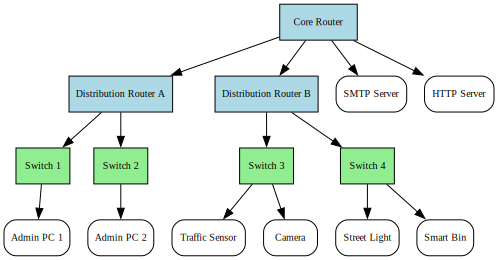
\includegraphics[width=\textwidth]{graphviz.png}
    \caption{Proposed Smart City IoT Network Architecture with IPv6 and QoS}
    \label{fig:network-diagram}
\end{figure}

\section*{Project Timeline}
\phantomsection
\addcontentsline{toc}{section}{Project Timeline}

\vspace{1em}
\renewcommand{\arraystretch}{1.2}
\setlength{\extrarowheight}{4pt}

\begin{center}
\begin{tabularx}{\textwidth}{
    |>{\raggedright\arraybackslash}p{2.4cm}
    |>{\raggedright\arraybackslash}p{4.2cm}
    |>{\raggedright\arraybackslash}X|
}
\hline
\textbf{Weeks} & \textbf{Phase} & \textbf{Key Activities} \\
\hline
Weeks 1--2 & Literature Review & Research smart city networks and IPv6 deployments \\
\hline
Weeks 3--4 & Project Planning & Finalize objectives, system design choices, and submit proposal \\
\hline
Weeks 5--6 & Network Design & Create detailed topology in Packet Tracer \\
\hline
Weeks 7--8 & Configuration & Implement IPv6, VLANs, and QoS policies \\
\hline
Weeks 9--10 & Testing & Validate failover capabilities and security configurations \\
\hline
Week 11 & Documentation & Compile findings, results, and technical report \\
\hline
Week 12 & Submission & Submit project files and deliver final presentation \\
\hline
\end{tabularx}
\end{center}

\section*{Expected Outcomes}
\phantomsection
\addcontentsline{toc}{section}{Expected Outcomes}
\begin{enumerate}[label=7.\arabic*, nosep]
    \item A fully functional smart city network supporting over 15 IoT devices
    \item Proven failover capability during router or link failures
    \item Verified QoS performance ensuring emergency traffic priority
    \item Comprehensive network documentation with step-by-step configuration templates
    \item Practical hands-on experience with advanced enterprise networking technologies
    \item A reference model adaptable to larger-scale real-world smart city deployments
\end{enumerate}

The results will confirm that IPv6 effectively addresses the connectivity, scalability, and performance requirements of modern smart cities.

\section*{Complex Engineering Problem Attributes}
\phantomsection
\addcontentsline{toc}{section}{Complex Engineering Problem Attributes}

\begin{center}
\renewcommand{\arraystretch}{1.2}
\begin{tabularx}{\textwidth}{|p{4.2cm}|X|}
\hline
\textbf{Attribute} & \textbf{How Project Meets It} \\
\hline
Conflicting Requirements & Efficiently allocating network bandwidth so emergency communications receive top priority while maintaining acceptable service quality for IoT devices and public users \\
\hline
Multiple Stakeholders & IoT sensors, city staff, administrative PCs, and public network users share infrastructure with differing needs \\
\hline
Depth of Analysis & Requires knowledge of IPv6 addressing, VLAN segmentation, ACL rules, and QoS policies \\
\hline
Extensive Knowledge & Combines advanced networking, security, and IoT integration concepts into a unified system \\
\hline
Interdependence & All network components, services, and configurations depend on each other for proper operation \\
\hline
\end{tabularx}
\end{center}

\section*{Limitations}
\phantomsection
\addcontentsline{toc}{section}{Limitations}
\begin{itemize}[nosep]
    \item \textbf{Simulation constraints:} Packet Tracer cannot perfectly replicate all real-world network conditions
    \item \textbf{Scale:} Limited to 15–20 devices compared to the thousands used in real cities
    \item \textbf{Wireless:} Unable to model actual interference and signal propagation complexities
    \item \textbf{Services:} Basic SMTP and HTTP functionality compared to production-grade platforms
    \item \textbf{Security:} No use of encryption or advanced cyber threat countermeasures
\end{itemize}

Despite these limitations, the prototype successfully demonstrates scalable concepts that can be expanded for real-world smart city networks.

\section*{Conclusion}
\phantomsection
\addcontentsline{toc}{section}{Conclusion}
This project addresses key networking challenges faced by modern smart cities through an IPv6-based IoT network design enhanced with QoS capabilities. The simulation showcases practical solutions for address exhaustion, prioritized traffic handling, and improved network resilience. By combining existing standards with thoughtful architecture, we present a blueprint for building efficient municipal sensor networks that enhance operational efficiency and emergency responsiveness.

The technical skills gained, along with the documented best practices, will be valuable for future deployments. While simulation limitations exist, the demonstrated concepts and configurations are directly applicable to larger-scale, production-grade smart city environments.

\end{document}
